\documentclass[11pt]{article}
\usepackage[utf8]{inputenc}
\usepackage{amssymb} %for fancy L
\usepackage{calrsfs} %for fancy L
\usepackage{cancel}
\usepackage{tabularx}
\usepackage[hyphens]{url}
\usepackage{booktabs}
\usepackage{graphicx}
\usepackage[titletoc,title]{appendix}
\usepackage{subfig}
\DeclareMathAlphabet{\pazocal}{OMS}{zplm}{m}{n} %for fancy L
\usepackage{epsfig, float,array,tabu,longtable,}
\usepackage{hyperref,wrapfig}
\usepackage{enumerate}
\usepackage{graphicx,psfrag}
\usepackage{cite}
\usepackage{sectsty}
\usepackage{epstopdf}
\usepackage{amsmath,esint, setspace, fancyhdr, amsfonts, bookmark, blindtext}
\usepackage[normalem]{ulem}
\usepackage{tikz}
\usepackage{rotating}
\usepackage[americanvoltages,fulldiodes,siunitx]{circuitikz}
\usepackage{stackengine}
\usetikzlibrary{matrix}
\usepackage{multirow}
\usepackage{multicol}
\usetikzlibrary{shapes,backgrounds,patterns}
\usetikzlibrary{mindmap,trees,decorations.markings}
\usetikzlibrary{quotes,angles}
\usepackage{verbatim}
\renewcommand{\baselinestretch}{1}
\setlength{\textheight}{8in}
\setlength{\textwidth}{6.5in}
\setlength{\headheight}{0in}
\setlength{\headsep}{0.25in}
\usepackage{graphicx}
\setlength{\topmargin}{0in}
\setlength{\oddsidemargin}{0in}
\setlength{\evensidemargin}{0in}
\setlength{\parindent}{.3in}
\usepackage{listings}
\usepackage{color} %red, green, blue, yellow, cyan, magenta, black, white
\definecolor{mygreen}{RGB}{28,172,0} % color values Red, Green, Blue
\definecolor{mylilas}{RGB}{170,55,241}
\doublespacing
\begin{document}


\begin{titlepage}

\newcommand{\HRule}{\rule{\linewidth}{0.5mm}} % Defines a new command for the horizontal lines, change thickness here
% Center everything on the page
 
%---------------------------------------------------------
%	HEADING SECTIONS
%---------------------------------------------------------
\center 
\newcommand*{\plogo}{
\includegraphics[width=0.25\textwidth]{./img/logo.png}}

\plogo \\[1.5 cm] % Include a department/university logo - this will require the graphicx package 

\textsc{\Large Software Atelier: Simulation, Data Science \& Supercomputing}\\[0.5cm] % Major heading such as course name
\textsc{\large Spring 2019 }\\[0.5cm] % Minor heading such as course title

%---------------------------------------------------------
%	TITLE SECTION
%---------------------------------------------------------

\HRule \\[1cm]
{ \huge \bfseries Image Segment Detection}\\[0.4cm] % Title of your document
\HRule \\[2.0cm]
 
%---------------------------------------------------------
%	AUTHOR SECTION
%---------------------------------------------------------



\begin{table}[h]
\centering
\begin{tabular}{l l}
\textbf{Liudmila Karagyaur} & {\href{mailto:karagl@usi.ch}{karagl@usi.ch}} \\
\textbf{Lorenzo Ferri} & {\href{mailto:ferril@usi.ch}{ferril@usi.ch}} \\
\textbf{Vanessa Braglia} & {\href{mailto:braglv@usi.ch}{braglv@usi.ch}} \\
\end{tabular}
\end{table}

%{\textsc{\textbf{Lorenzo Ferri}}} 	\quad\quad \quad\quad{\href{mailto:ferril@usi.ch}{ferril@usi.ch}}\\
%{\textsc{\textbf{Vanessa Braglia}}} 	\quad\quad \quad{\href{mailto:braglv@usi.ch}{braglv@usi.ch}}\\


~
%\begin{minipage}{0.4\textwidth}
%\begin{flushright} \large
%\emph{Supervisor:} \\
%Dr. James \textsc{Smith} % Supervisor's Name
%\end{flushright}
%\end{minipage}\\[4cm]

% If you don't want a supervisor, uncomment the two lines below and remove the section above
%\Large \emph{Author:}\\
%John \textsc{Smith}\\[3cm] % Your name

%---------------------------------------------------------
%	DATE SECTION
%---------------------------------------------------------
\begin{center}
{\large \today}
\end{center}
 % Date, change the \today to a set date if you want to be precise

%---------------------------------------------------------
%	LOGO SECTION
%---------------------------------------------------------
%\vfill
%\newcommand*{\plogo}{
\includegraphics[width=0.25\textwidth]{./img/logo.png}}
%
%\plogo\\[1cm] % Include a department/university logo - this will require the graphicx package
 
%---------------------------------------------------------

\vfill % Fill the rest of the page with whitespace
\end{titlepage}

\newpage
\tableofcontents
\newpage

% EXECUTIVE SUMMARY %%%%%%%%%%%%%%%%%%%%%%%%%%%%%%%%%
\addcontentsline{toc}{section}{Introduction}
\section*{Introduction}
Nowadays edge detection techniques have several applications. For example,  a content based video retrieval is widely required for searching digital information in large databases, in order to improve text based retrieval systems \cite{1}. It also has an important role in the development of self-driving vehicles, that need to perform a real-time feature detection \cite{2}, and in medical field, in the analysis of digital images of pathological conditions, such as tumors \cite{3}.    \\
The ultimate goal of this project is to find the main features in a video and to be able to follow their trajectories. In particular, we will analyse single video frames using edge detection, which is an image segmentation technique.  \\
There exists a great variety of clustering algorithms that can perform an efficient image segmentation, which is a fundamental step in feature extraction.  The first step consists in analysing different clustering algorithms and detect the most suitable one to the problem at hand. \\
Since the frames could be noisy or blurry, the next stage will focus on possible ways to improve the result of the clustering algorithm, by looking for an optimal sharpening operator. In this step some deblurring techniques will be examined. \\
Finally, the edge detection will be executed in parallel on each frame of the video, in order to improve the performance. 

\newpage
\section{Project tasks}
\subsection{Image clustering}
Clustering ia a technique that allows, given a dataset of points, to classify them into different groups depending on their features. In our case the datapoints that have to be classified are the pixels of the given image. The  algorithms that will be examined are k-means, DBSCAN and spectral clustering. 
\subsubsection{k-means}
The k-means algorithm is the simpliest and the most popular clustering algorithm. Its ultimate goal is to partition $n$ initial datapoints into $k$ clusters. It requires that the user provides the number $k$ of clusters that have to be found. The algorithms uses an iterative techniques:,starting from an initial set of random centroids. At each iteration it generates the clusters by minimizing the Euclidean distance $D$ between each point $x_i$  and  the centroids $c_j$:  
$$\arg \min\limits_{j}D(x_i, c_j)\;\;\;\; j = 1, \dots, k$$
Then, for each cluster $C_j$ a new centroid $c_j$ is computed as the mean of all $n_j$ points $x_i$ assigned to the cluster in the previous step: 
$$c_j = \frac{1}{n_j} \sum_{x_i \in C_j} x_i$$

\subsubsection{DBSCAN}
Density-Based Spatial Clustering of Applications with Noise algorithm needs two parameters in order to perform clustering on data: the maximum radius (\textit{eps}) of the neighbourhood and the minimum number of points (\textit{MinPts}) in the \textit{eps}-neighbourhood of a point. All the points are classified as: 
\begin{itemize}
	\item \textbf{core point}: if it has equal or more than \textit{MinPts} points in its  \textit{eps}-neighbourhood 
	\item \textbf{border point}: if it has less than \textit{MinPts} points in its  \textit{eps}-neighbourhood, but it is in the neighbourhood of a core point
	\item \textbf{noise point}: any point that is not a core or a border point.
\end{itemize} 
Then the datapoints are assigned to clusters in the following way. Any two core points that belong to each other's neighbourhood (located within a distance \textit{eps}) are assigned to the same cluster; any border point that belongs to the \textit{eps}-neighbourhood of a core point is assigned to the same cluster of the core point. Noise points are discarded. 

\begin{figure}[h]
	\centering
	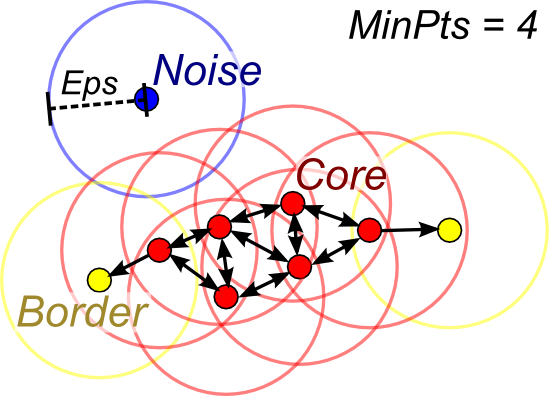
\includegraphics[width=0.4\linewidth]{dbscan}
	\caption{An illustration of DBSCAN algorithm}
	\label{fig:dbscan}
\end{figure}

\subsubsection{Spectral clustering}


\subsection{Image deblurring}
\subsection{Feature extraction}


\begin{thebibliography}{9}
	
	\bibitem {1}
	B.V. Patel and B.B. Meshram,
	\textit{Content Based Retrieval Systems},
	International Journal of UbiComp (IJU), Vol.3, No.2, 
	April 2012
	
	\bibitem {2} 
	H. Cho, Y. Seo, B. V. K. V. Kumar and R. R. Rajkumar, 
	\textit{A multi-sensor fusion system for moving object detection and tracking in urban driving environments}, 
	IEEE International Conference on Robotics and Automation (ICRA), 
	2014

	\bibitem {3} 
	Ed-Edily Mohd,  Azhari,Muhd. Mudzakkir Mohd. Hatta1, Zaw Zaw Htike1andShoon Lei Win, 
	\textit{Tumor detection in medical imaging: a survey }, 
	International Journal of Advanced Information Technology (IJAIT) Vol. 4, No. 1, 
	February 2014
	
	
	
\end{thebibliography}


\end{document}